
%(BEGIN_QUESTION)
% Copyright 2012, Tony R. Kuphaldt, released under the Creative Commons Attribution License (v 1.0)
% This means you may do almost anything with this work of mine, so long as you give me proper credit

A high-voltage circuit breaker is manually operated from a remote location using a pair of pushbutton switches, connected to ``trip'' and ``close'' solenoid coils within the breaker:

$$\includegraphics[width=15.5cm]{i01894x01.eps}$$

Note: the ``52a'' and ``52b'' contacts wired in series with the solenoid coils within the breaker are {\it auxiliary} contacts, actuated by the same mechanism as the three power contacts (i.e. 52a contacts are open when the power contacts are open, and closed when the power contacts are closed.  52b contact always exhibits the opposite state as the power contacts).  The two trip coils are redundant: only one of them needs to energize in order to trip the circuit breaker.

\vskip 10pt

Given the following dependability figures for each component, and assuming all other elements in the system are 100\% reliable, calculate the probability of failure for breaker tripping (i.e. the probability that the breaker will {\it not} trip when the ``Trip'' pushbutton is pressed), and also the probability of failure for breaker closing (i.e. the probability that the breaker will {\it not} close when the ``Close'' pushbutton is pressed).

\begin{itemize}
\item{} Pushbutton contact = 0.991 (each) \hskip 50pt PFD$_{close}$ = \underbar{\hskip 50pt}
\item{} Coil = 0.99987 (each)
\item{} Fuse = 0.9971 (each) \hskip 100pt PFD$_{trip}$ = \underbar{\hskip 50pt}
\item{} Battery = 0.9984
\end{itemize}

\vskip 20pt \vbox{\hrule \hbox{\strut \vrule{} {\bf Suggestions for Socratic discussion} \vrule} \hrule}

\begin{itemize}
\item{} Which function, tripping or closing, has the least probability of failure?  Why do you think the system is designed this way?
\item{} What is the purpose for having auxiliary contacts in the trip and close circuits?
\end{itemize}

\underbar{file i01894}
%(END_QUESTION)





%(BEGIN_ANSWER)

\noindent
{\bf Partial answer:}

\vskip 10pt

Probability calculation for ``closing'' PFD using logic symbols:

$$\includegraphics[width=15.5cm]{i01894x02.eps}$$

%(END_ANSWER)





%(BEGIN_NOTES)

Probability calculation for ``tripping'' PFD using logic symbols:

$$\includegraphics[width=15.5cm]{i01894x03.eps}$$

\vskip 20pt \vbox{\hrule \hbox{\strut \vrule{} {\bf Virtual Troubleshooting} \vrule} \hrule}

This question is a good candidate for a ``Virtual Troubleshooting'' exercise.  Presenting the diagram to students, you first imagine in your own mind a particular fault in the system.  Then, you present one or more symptoms of that fault (something noticeable by an operator or other user of the system).  Students then propose various diagnostic tests to perform on this system to identify the nature and location of the fault, as though they were technicians trying to troubleshoot the problem.  Your job is to tell them what the result(s) would be for each of the proposed diagnostic tests, documenting those results where all the students can see.

During and after the exercise, it is good to ask students follow-up questions such as:

\begin{itemize}
\item{} What does the result of the last diagnostic test tell you about the fault?
\item{} Suppose the results of the last diagnostic test were different.  What then would that result tell you about the fault?
\item{} Is the last diagnostic test the best one we could do?
\item{} What would be the ideal order of tests, to diagnose the problem in as few steps as possible?
\end{itemize}

\vskip 20pt \vbox{\hrule \hbox{\strut \vrule{} {\bf Virtual Trip-testing} \vrule} \hrule}

This question is a good candidate for a ``Virtual Trip-testing'' exercise.  Presenting the diagram to students, you pose an assignment whereby students must figure out how to test some component of this system to check that it will operate as intended to shut down the system in an abnormal (trip) condition, with some realistic limitation (e.g. power cannot be shut off to the load).  Students then propose various methods for executing the test.  Your job is to determine whether or not their proposed tests will achieve the desired result(s).

During and after the exercise, it is good to ask students follow-up questions such as:

\begin{itemize}
\item{} Where might our planned test strategy go wrong?  In other words, what thing(s) might happen to foil our test, either to invalidate the results or to not honor the stated limitation(s)?
\item{} Suppose the limitation were different.  How would this affect our ability to carry out the test?
\item{} Is the last test strategy best one we could execute?
\end{itemize}


%INDEX% Electric power systems: HV circuit breaker controls
%INDEX% Safety, system reliability: probability of reliable operation
%INDEX% Safety, system reliability: probability of failure on demand (PFD)

%(END_NOTES)


